\begin{figure}[!t]
\centering
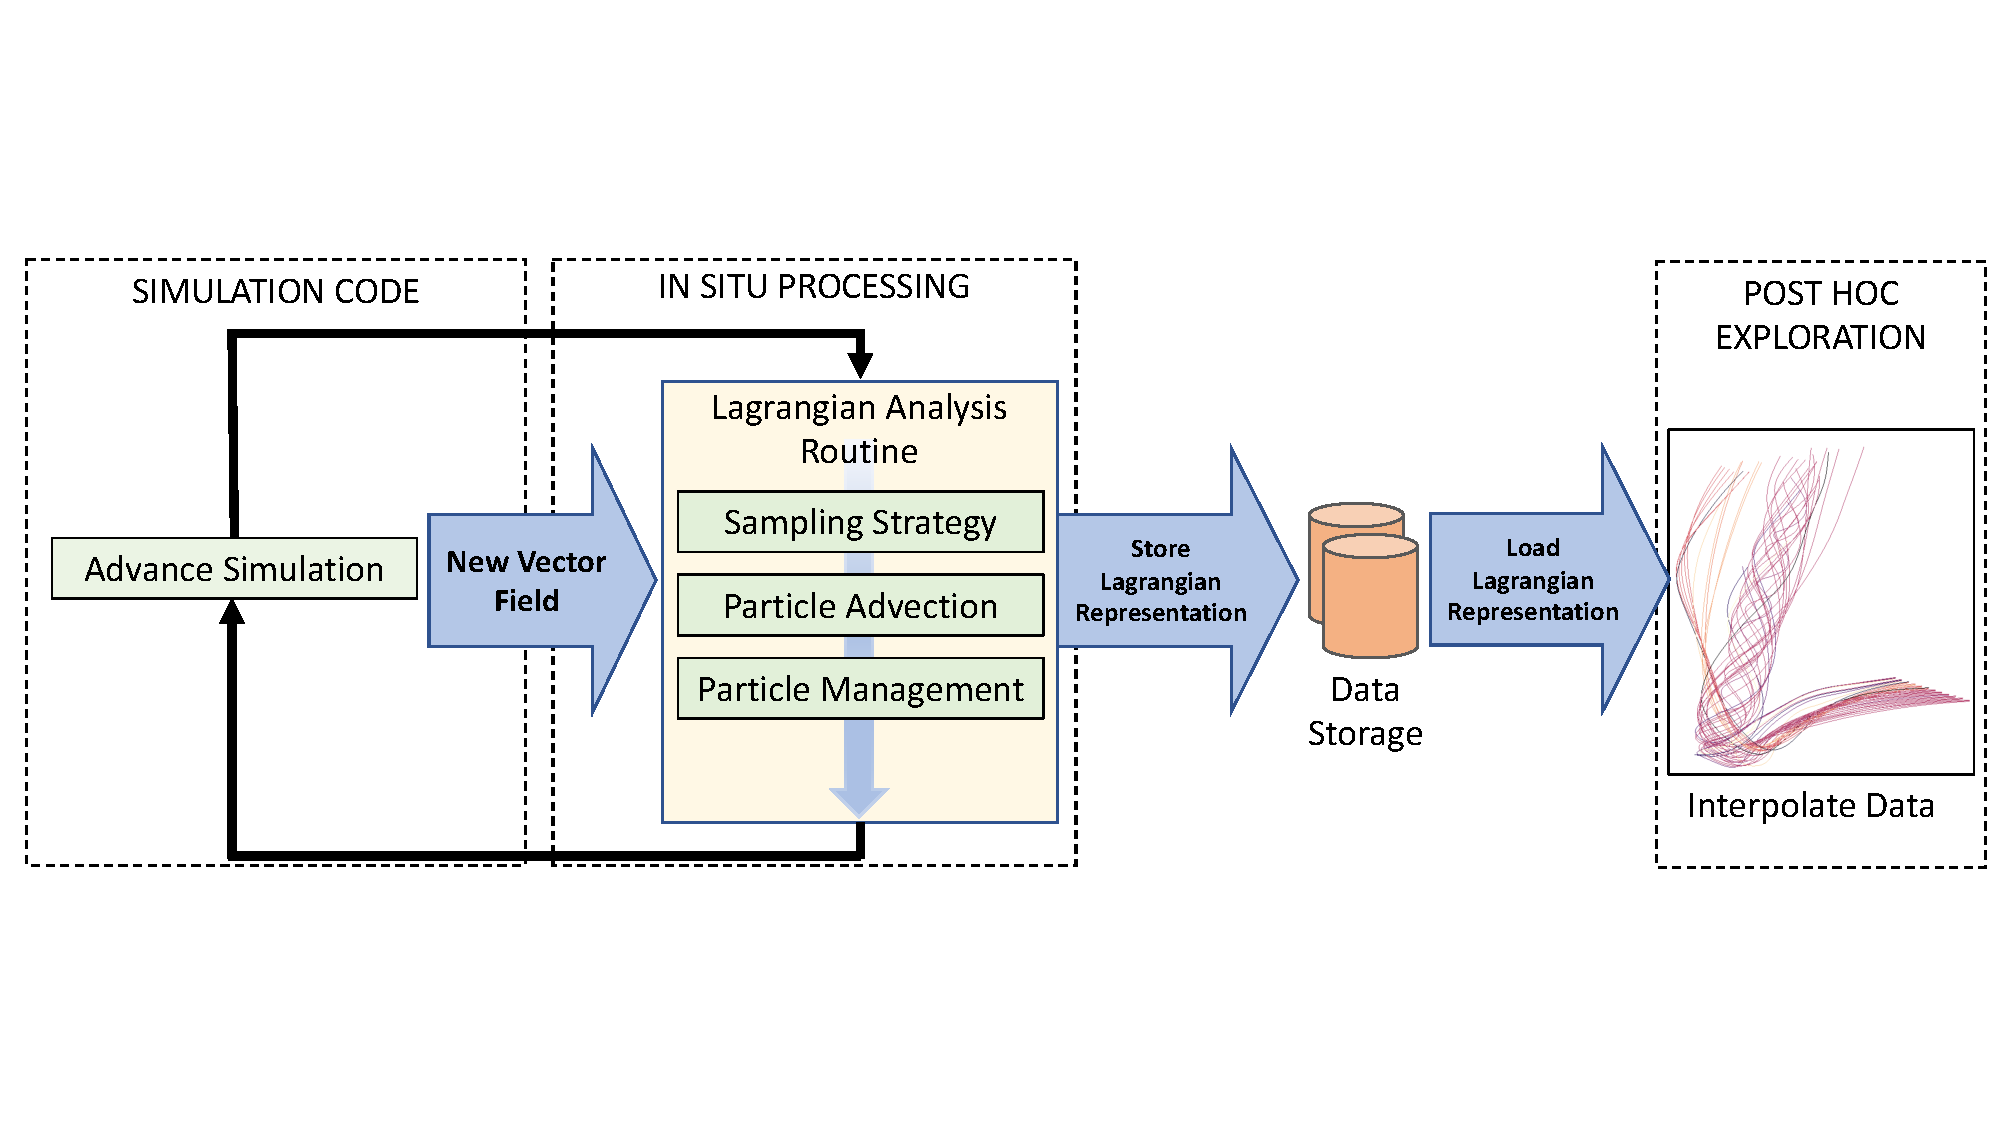
\includegraphics[width=0.9\linewidth,trim={0cm 4.3cm 0cm 4.3cm}, clip ]{Images/Schematic.pdf}
\vspace{-2mm}
\caption{Schematic diagram of the Lagrangian in situ reduction and post hoc exploration workflow showing the simulation code with in situ processing integrated, data storage, and post hoc analysis.}
\vspace{-5mm}
\label{fig:schematic}
\end{figure}

%This section describes considerations for using and evaluating Lagrangian in situ reduction (L-ISR) for cosmology and seisomology time-varying vector fields. Specifically:
%\begin{tightItemize}
%\item Subsection~\ref{sec:instantiation} describes the instantiation we consider.
%\item Subsection~\ref{sec:evaluation} describes important evaluation criteria.
%\item Subsection~\ref{sec:workloads} describes important factors in defining workloads.
%\end{tightItemize}
%
%\subsection{Instantiation}
%\label{sec:instantiation}

This section describes the instantiation we consider for our study.
%
Figure~\ref{fig:schematic} shows a high-level description of the Lagrangian in situ reduction post hoc exploration (L-ISR-PHE) workflow. 
%
There are many possible strategies for accomplishing the components within this workflow.
%
For our study, we focus on the current best practices in this space.
%
To describe our instantiation, the remainder of this section is divided based on two phases: in situ reduction and post hoc exploration. 
%
\subsubsection{In Situ Reduction}
In the in situ phase, as a data reduction operator without any a priori knowledge, a good strategy is to place samples such that domain coverage is maintained.
%
We compute multiple temporally non-overlapping sets of massless particle trajectories over the duration of the simulation.
%
We refer to these trajectories as \textit{basis} trajectories.
%
Each set of basis trajectories encodes the behavior of the time-varying vector field over a specific interval of time.
%
To introduce particles at the start of an interval, we use the uniform seed placement scheme by Agranovsky et al.~\cite{agranovsky2014improved}. 
%
Using a uniform placement and resetting the particle trajectories after an interval helps maintain domain coverage and is simple to implement.
%
Our particle termination follows the local Lagrangian flow map model from Sane et al.~\cite{sane2020scalable}, where particles are terminated once they reach the end of the interval or exit the block.
%
Our implementation has two main knobs that control the total data storage and quality of reconstruction: number of basis trajectories, i.e., seed resolution, and frequency of storing information to disk, i.e., storage interval.
%
The effect of these settings varies depending on the underlying vector field. 
%
%We discuss these in~\ref{sec:workloads}.

We use the Ascent~\cite{larsen2017alpine} in situ infrastructure and VTK-m~\cite{moreland2016vtk} library to implement L-ISR. 
%
The Ascent API can be used to integrate with an application code and access various in situ analytics capabilities.
%%
The VTK-m Lagrangian filter on each rank operates independently and maintains its own list of particles and uses the existing particle advection infrastructure available in VTK-m~\cite{pugmire2018performance}.
%
RK4 particle advection is implemented using VTK-m worklets (kernels or functors) that offer performance portability by utilizing the underlying hardware accelerators.
%
In our implementation, each Lagrangian filter stores the displacement of each particle (3 double), as well as its validity (1 boolean), i.e., whether the particle remained within the domain during the interval of calculation.
%
Overall, computing a Lagrangian representation increased the runtime memory cost on the simulation by approximately by four one-dimensional simulation ``fields''.
%
We note that simulations can have tens to hundreds of fields defined on the simulation grid and thus, this cost would likely be considered acceptable for most simulations.
%
In more complicated frameworks, it is possible to associate additional information (for example, ID, age, start location, previous locations, etc.) with each particle at the cost of higher runtime memory usage and data storage.
%

To compute a Lagrangian representation, the simulation has to invoke Ascent after every cycle it advances.
%
Ascent accesses the simulation vector field data and consequently invokes the Lagrangian filter. 
%
The Lagrangian filter uses the vector field to advance particles, and triggers the storage of trajectories at the end of an interval.
%
%In our implementation, following previous work~\cite{agranovsky2014improved}\cite{sane2018revisiting}\cite{sane2020scalable}, a trajectory in the Lagrangian representation is stored using a start and end location.
%
All the steps from creating an instance of Ascent to specifying parameters and invoking the VTK-m Lagrangian filter require only 23 lines of code (C++) and less is a JSON input file is used.
%
%The code sample below shows an Ascent integration and invocation of the Lagrangian filter in C++. 
%
%\begin{lstlisting}[basicstyle=\small, language=C++] 
%Ascent ascent;
%Node ascent_opts;
%ascent_opts[``runtime/type''] = ``ascent'';
%ascent.open(ascent_opts);
%conduit::Node mesh_data;
%// Populate mesh_data;
%conduit::Node pipelines;
%// pipeline 1
%pipelines[``pl1/f1/type''] = ``lagrangian'';
%// filter knobs
%conduit::Node &lagrangian_params = pipelines[``pl1/f1/params''];
%lagrangian_params[``field''] = ``velocity'';
%lagrangian_params[``step_size''] = 0.02; 
%lagrangian_params[``storage_interval''] = 25; 
%lagrangian_params[``seed_resolution''] = 8; 
%conduit::Node actions;
%// add the pipeline
%conduit::Node &add_pipelines = actions.append();
%add_pipelines[``action''] = ``add_pipelines'';
%add_pipelines[``pipelines''] = pipelines;
%// execute
%conduit::Node &execute  = actions.append();
%execute[``action''] = ``execute'';
%// reset
%conduit::Node &reset  = actions.append();
%reset[``action''] = ``reset'';
%ascent.publish(mesh_data);
%ascent.execute(actions);
%ascent.close();
%\end{lstlisting}
%
%
%We use Ascent to store the complete velocity field at a specified frequency in order to evaluate the traditional Eulerian paradigm.
%
%For every Eulerian configuration, we store the full spatial resolution of the simulation domain under consideration.
%
%
\subsubsection{Post Hoc Exploration}
For post hoc analysis, new particle trajectories can be computed by interpolating basis trajectories that were extracted in situ.
%
The essential operations involved in constructing new particle trajectories are identifying which basis trajectories to follow and then performing interpolation.
%
Based on the study of accuracy of various Lagrangian-based advection schemes in~\cite{agranovsky2015subsampling}, our study employs a Delaunay triangulation to identify the neighborhood of valid basis trajectories and second-order barycentric coordinates interpolation.
%
We used the CGAL~\cite{fabri2011cgal} library to construct and search the Delaunay triangulation.
%
After reconstructing new pathlines or deriving new scalar fields from the data extracted in situ, we use VisIt~\cite{childs2012visit} to generate visualizations.
%\subsection{Evaluation Criteria}
%\label{sec:evaluation}
%In this study, we consider the following four evaluation criteria (EC) across the workflow:
%%
%\begin{tightEnumerate}
%\item\textbf{(EC1) In situ reduction time:} the execution time spent by the simulation on data analysis and visualization.
%\item\textbf{(EC2) In situ reduction memory:} the runtime memory used by in situ processing.
%\item\textbf{(EC3) Data storage size:} the file storage costs (i.e., bytes).
%\item\textbf{(EC4) Post hoc exploration accuracy:} the quantitative and qualitative accuracy of new interpolated trajectories or derived fields.
%\end{tightEnumerate}
%%
%
%\subsection{Workload Factors}
%\label{sec:workloads}
%To understand the performance characteristics of L-ISR, we identified four parameters that when varied produce the workloads we want to evaluate for our study:
%\begin{tightEnumerate}
%\item\textbf{(WF1) Number of basis particles:} 
%%We vary the number of basis particles initialized per rank. The number of basis trajectories impacts the cost of particle advection every cycle of the simulation, the size of the data stored to disk and the accuracy of the reconstruction. 
%%
%We specify the number of particles initialized using the notation $\textbf{1:X}$, where X is the reduction factor. For example, a 1:8 configuration states that one particle is used for every 8 grid points (12.5\% of the original data size). WF1 impacts every EC.
%\item\textbf{(WF2) Storage interval:} 
%%We consider the frequency at which files are stored to disk. Additionally, for the Lagrangian representation, the interval is equal to the integration length of each particle, and can thus, be consequential to the accuracy of reconstruction. 
%%
%We use $\textbf{I}$ to denote storage interval. WF2 impacts EC3 and EC4. 
%\item\textbf{(WF3) Grid size:} 
%%We consider different grid sizes to measure the in situ encumbrance of varying workloads. In particular, we are interested in the in situ encumbrance when a single compute node is operating on a large number of grid points. An additional benefit of varying the grid size is insight into the variation in simulation cycle time and consequently the percentage of time spent on in situ processing. 
%WC3 impacts EC1, EC2, and EC3. 
%\item\textbf{(WF4) Concurrency:} We consider the costs at multiple scales (i.e., number of compute nodes, MPI ranks). Further, the simulation codes described in \ref{sec:simulations} required different parallelization hardware, and thus, between simulation codes we measure the costs of Lagrangian representation extraction using, both, GPUs and CPUs for particle advection. WF4 impacts EC1 and EC2.
%\end{tightEnumerate}
